\documentclass[12pt, a4paper]{article}

\usepackage{graphicx, color}
\usepackage{geometry}
\usepackage{multirow}
\usepackage{sectsty}
\usepackage{amssymb}
\usepackage{wrapfig}
%\usepackage{natbib}
\usepackage{hyperref}
\usepackage{float}

\begin{document}
\title{\color{red} The Lazy Man's Cycle Starter}
\maketitle

\begin{table}[ph]
\large
\centering
\begin{tabular}{c c c}
\hline
GroupName &RollNumber &Name\\
\hline 
\multirow{3}{*}{!JustCoders} &140050031 &C Vishwesh\\ &140070003 &Saurabh Garg\\&140070031 &Aviral Kumar\\
\hline
\end{tabular}
\end{table}

\newpage
\vspace*{\fill}
\begin{center}
{\textbf{HONOR CODE}}\\
\textit{"I pledge on my honour that I have not given or received any unauthorized assistance on this assignment or any previous task."}\\
\end{center}
\vspace*{\fill}
\pagebreak

\addcontentsline{toc}{section}{Introduction}
\section{Introduction}
\subsection{Purpose}
This project has been done as a part of the course CS 251 : Software Systems Lab offered to CS Majors at IIT Bombay in the second year. This SRS cum Report gives a semi-detailed description and the specific software requirements for running our Project.

\subsection{Scope}
\begin{list}{$\cdot$}{\leftmargin=3.5em}
\item[-] {This is a project aimed at making a \textbf{Rube Goldberg Machine} in the Box2D environment}
\item[-] {The software basically simulates a Rube Goldberg Machine by the name \textbf{\textit{Lazy Man's Cycle Starter}}}
\item[-] {
The applications of the software are: 
	\begin{list}{-}{\leftmargin=2em}
		\item[-] {It provides a simulation which is interesting to look at.}
		\item[-] {The software can be extended to add more complexities and a much trickier path.}
	
	\end{list}	  
}
\end{list} 

\subsection{Overview}
The rest of the SRS contains a brief and a detailed description of the software including the requirements which need to be fulfilled to be able to run the software on the system and develop it furthur.

\pagebreak
\section{General Description}
\subsection{Product Perspective}
Many other projects have been and are being made in box2d in the past and present respectively. The difference between all such projects comes when the idea behind the simulation is taken into account. The idea of this project i.e. the storyline of this project is what makes it different from the rest of the projects.  

\subsection{Product Functions}
The product will basically give the user an opportunity to pull down a block which would trigger the chain reaction involved in the simulation, and the simulation will then go ahead as planned.

\subsection{User Characteristics}
The user should not pull the string to fast or too slow, or else the code will show some interesting collisions and some interesting random results.   

\subsection{General Constraints}
Giving the user mouse-joint facilities can lead to some random results sometimes, so the user should pull the rope in a sensible manner.

\subsection{Assumptions and Dependencies}
The SRS document assumes that the system on which the software is being run has g++ complier and Box2D is installed on the machine. Moreover OpenGL should also be installed on the machine. If not please refer to the Box2D and(or) OpenGL installation guide(s). Moreover, like any video game, any random input could lead to random results in the simulation.

\pagebreak
\section{The "Ram Katha" of the Project}

\subsection{What we planned to do}
\begin{list}{$\cdot$}{\leftmargin=3.5em}
\item[-] {Make a Rube Goldberg Machine which could make a lazy man stuck on a cycle with square shaped wheels, on a road made of Catenary curves move without making any effort}
\item[-] {The man pulls a string which initiates a mechanical chain reaction finally resulting in the above}
\item[-] {The elements include a stack of 2-dominos (one domino placed over the other), a spring-mass (2 bodies connected by a spring) system, a two-pulley system (Two pulleys sharing one common rope), Catenary curves, balloon, hourglass, Newton's pendulum, a cut-rope system(a joint breaks when a collision occurs), funnel, bicycle, rotating turbines, etc }
\end{list}


\subsection{What we actually did}
\begin{list}{$\cdot$}{\leftmargin=3.5em}
\item[-] {We completed the main stuff we had proposed to do. We had maintained a local git repo individually on our computers as our parts were disjoint and then we finally integrated and maintained the new code.}
\item[-] {We had initially planned to make 2 pendulums and a few planks in the left part of the system but we replaced it with a spiral (Helix) and Newton's pendulum. We did this so as to make the system more complex and to fill up the space that would have arisen in the earlier system.}
\item[-] {We adjusted the slopes of the two planks on which the spring mass system was to be kept so as to make the chain reaction possible without any problem.}
\item[-] {We increased the number of rotating turbine like structures to two to facilitate the ball to go into the spiral path.} 
\end{list}
\subsection{Our work plan}
\begin{list}{$\cdot$}{\leftmargin=3.5em}
\item[-] {We divided the work into making objects and then integrated the work done by the three of us.}

\item[-] {Vishwesh made the spiral (Helix), catenary curves, bicycle, cut-rope system debugging, etc.}
\item[-] {Saurabh made the spring mass system, domino stack, balloon, funnel, hourglass, etc.}
\item[-] {Aviral made the Newton's pendulum, 2-pulley system, hourglass, the cut-rope mechanism, mouse joint, etc.}
\item[-] {The integration of the project was done by Saurabh (Major), Aviral(Minor) and Vishwesh (Minor)}
\item[-] {All of us documented the individual parts of the code.}
\item[-] {Report and presentation were made by Aviral.}
\item[-] {Website was made by Vishwesh.}
\item[-] {Profiling was done by Saurabh.}
\end{list}

\subsection{Difficulties we faced}
\begin{list}{$\cdot$}{\leftmargin=3.5em}
\item[-] {Making a pulley system with two pulley joints sharing one common rope required the definiton of a new joint (as per the Web search results) and we spent considerable amount of time thinking on how this had to be done. But we finally came up with a clever solution (of making an object common to both the pulley systems and setting its gravity to be zero) \textbf{Resolved}}
\item[-] {Making a spriral was also difficult as it involved a bit of math and a slightly longer code \textbf{Resolved}}
\item[-] {Making of the cut-rope system(i.e. ropes holding a piece of the Catenary curve break when it collides with a ball) turned out to be the most difficult part of the project as this kind of event handling didn't work out well using any of the options tried. But finally we were able to implement it. \textbf {Resolved}}
\item[-] {Integration of code was also an issue where we had to think and give a lot of time.}
\item[-] {The output also depended on the time at which the user pulled the string down. Making the simulation certain to happen was a challenging task and we made it finally.}
\item[-] {This is not a challenge related to making the project. But one of our teammates lost his whole work due to rm -rf ~/ which ran due to some mistake and we lost some of the changes in our code and this made us submit late by 1 day as we had to redo it once again.} 
\end{list}

\subsection{Project Details}
\begin{figure}[H]
\caption{Screenshot of the working project}
\centering
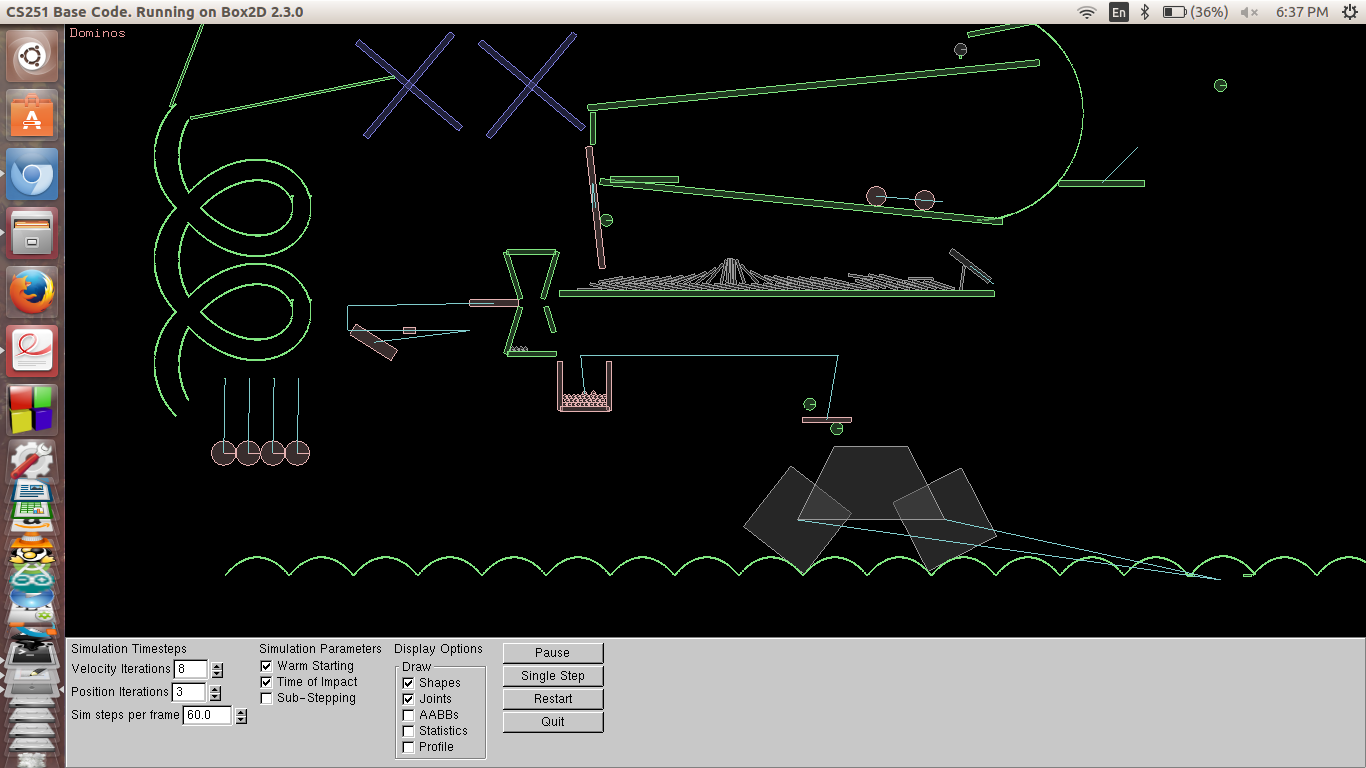
\includegraphics[scale=0.30]{screenshot.png}
\end{figure}
\subsubsection{Components}
Some of the major components in our simulation are:
\begin{enumerate}
\item \textbf{Helix} - This is a roller-coaster like path through which the ball goes. We made this using the equation of the spiral which we found on the web. 
\begin{figure}[H]
\caption{Helix}
\centering
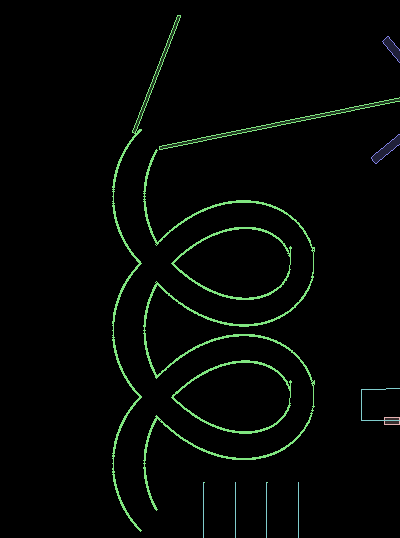
\includegraphics[scale=0.20]{helix.png}
\end{figure}
\item \textbf{Catenary curves} - These are special type of curves whose equation is given by $y= cosh(\frac{x}{a})$. A square can smoothly move through a chain of these curves if the perimeter of the sqaure and the length of one cycle of the catenary curve matches.
\begin{figure}[H]
\caption{Catenary curve Path}
\centering
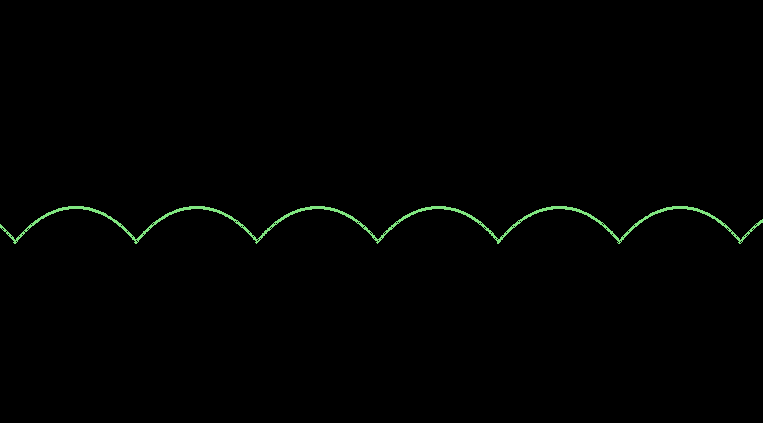
\includegraphics[scale=0.20]{catenary2.png}
\end{figure}
\item \textbf{Bicycle} - We have simulated a bicycle by using a trapezium and two squares for wheels. The trapezium and squares have a revolute joint in between them.
\begin{figure}[H]
\caption{Newton's Pendulum and Bicycle}
\centering
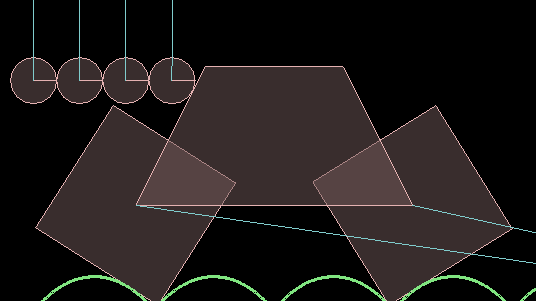
\includegraphics[scale=0.3]{pendulum.png}
\end{figure}
\item \textbf{Cut-Rope System} - A catenary curve (one cycle of it) is hanging from a rope above. Directly below it the road has a deep hole (a hole in the road exists). The simulation makes the part of the road (Catenary curve) fall and complete the road so that the bicycle is able to move on it without any interruption.
\begin{figure}[H]
\caption{Cut Rope System}
\centering
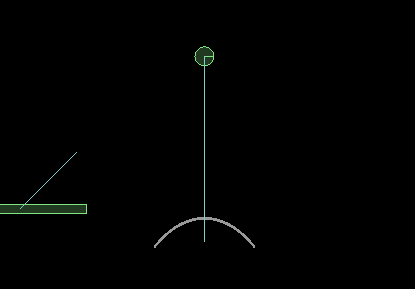
\includegraphics[scale=0.30]{path.png}
\end{figure}
\item \textbf{Spring Mass System} - Two bodies are connected by a spring in between which can extend and compress (just like a spring, this is defined by a prismatic joint, although it doesn't look like one).
\begin{figure}[H]
\caption{Spring Mass system}
\centering
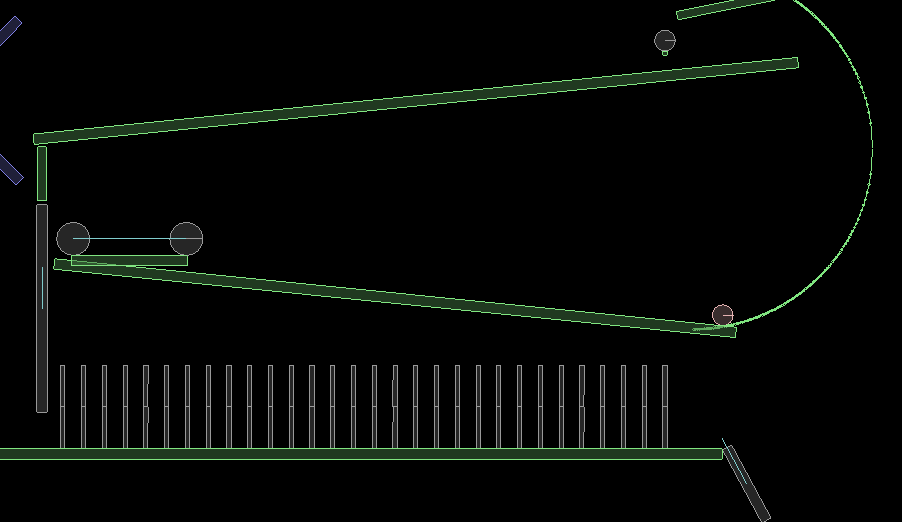
\includegraphics[scale=0.20]{springmass.png}
\end{figure}
\item \textbf{Two pulley system} - This is a system of two pulleys, one horizontal and the other vertical both of which share a common edge. This has been done by making a body attached to both the pulleys and setting its gravity to zero, so that it doesn't fall down.
\begin{figure}[H]
\caption{Two-pulley system}
\centering
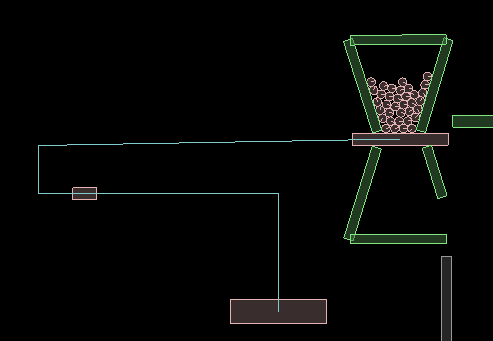
\includegraphics[scale=0.25]{2pulley.png}
\end{figure}
\item \textbf{Fans/Turbines} - These two systems of turbines facilitate the motion of the ball into the roller coaster like helix so that the whole simulation can occur without any difficulty.
\begin{figure}[H]
\caption{Fans}
\centering
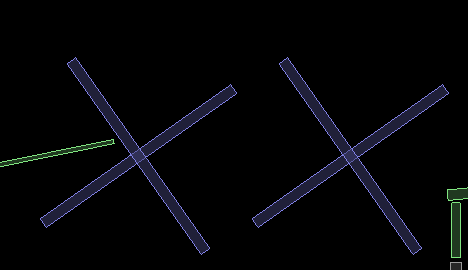
\includegraphics[scale=0.25]{fans.png}
\end{figure}
\item \textbf{Hourglass} - Initially the upper part of the hourglass is filled with water and when the user pulls the plank out, it falls down into the empty container nearby starting the chain reaction.    
\begin{figure}[H]
\caption{Hourglass}
\centering
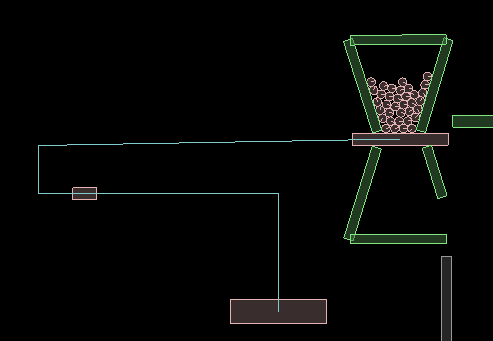
\includegraphics[scale=0.30]{pulleyandhourglass.png}
\end{figure}
\end{enumerate}
%The screenshot of the project screen and individual components is there below.
%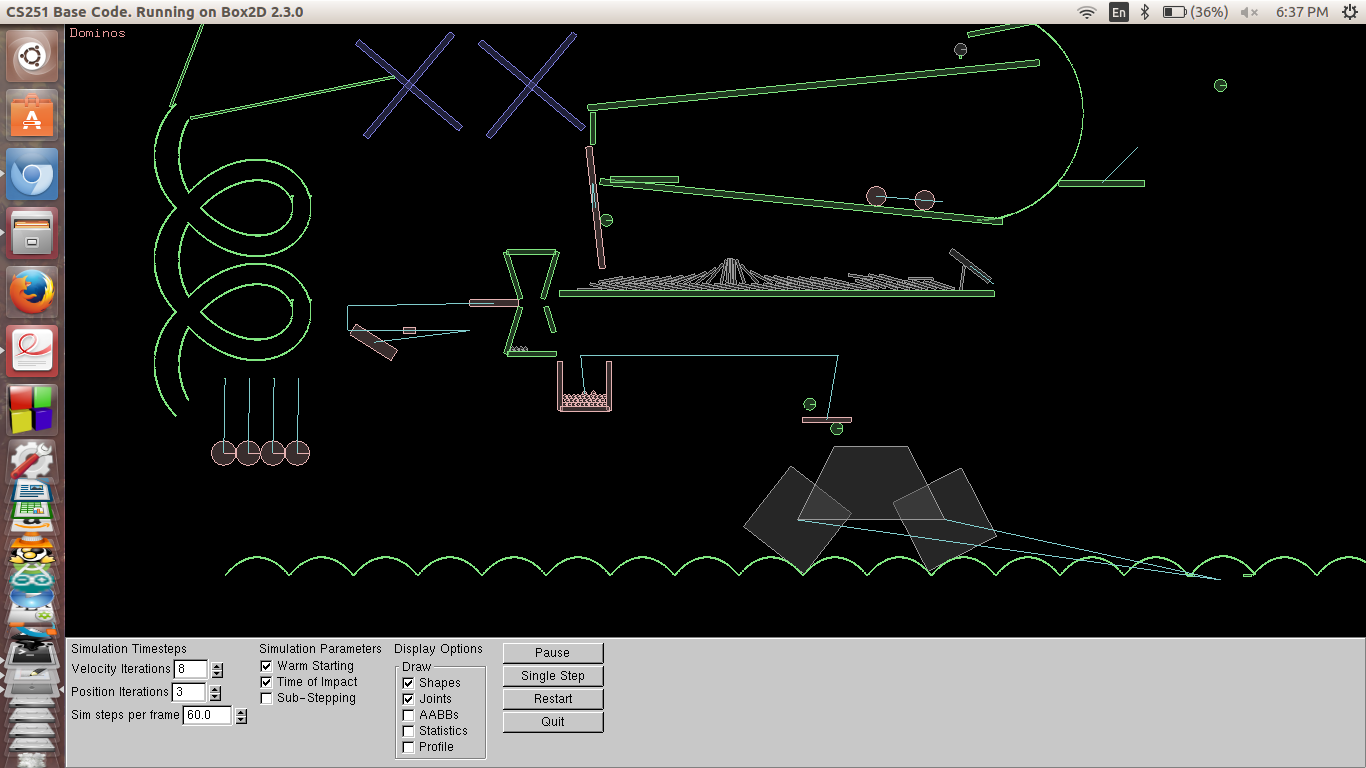
\includegraphics[scale=0.3]{screenshot.png}


\subsubsection{Working}
\begin{enumerate}
\item {The man sitting on the cycle pulls the rope hanging in front of him
downwards (this has been implemented by providing the user the
chance to pull the rope down) which triggers a chain reaction.}

\item {The balloon gets freed and moves up, hits the rod connected by a
hinge to the plank on which the dominos are kept. This rod hits the
dominos which fall down one by one giving a nice visual effect.}

\item  {Energy is transfered to the left end of this plank and then to the spring mass
system, which hits a ball that starts moving up after that. There's a plank above gthis ball too, which is "active" state. The ball which goes into the spiral helix is prevented from moving by a small barrier. When that ball hits the plank, it gets deactivated (it eats up the ball and deactivates itself!!) which removes the barrier and frees the other ball. }

\item {This ball crosses over the fans/ turbines and enters the spiral helix path, finally leaving it and hitting the Newton’s pendulum, which then  hits the cycle and brings it into motion.}

\item {Meanwhile, on the other side, the balloon hits the hanging catenary cuve which is pointed, and this leads to bursting of the balloon. Due to the impulse creagted by this, the rope holding the Catenary curve breaks off. The curve falls down and completes the road.}
\end{enumerate}

\subsection{Interesting facts}
The idea behind the simulation, the storyline of the simulation itself is quite interesting and new in itself. Moreover, because we have provided the user a facility to initiate the chain reaction, final outputs might differ time to time. (For example, we tried, infact played with it many times, and it worked perfectly almost two third number of times. Weird user inputs gave weird output results sometimes.)

\section{Profiling Data}
We have done some optimisations and dominos.cpp was significantly changed. In this optimised code of our project, debug\_ draw\_ t :: 
 (i.e. it took the most time) whereas in the original code, b2World::DrawDebugData() was the highest time consumer. The images of the call graph are (We cut the image into multiple parts and put them):

\subsection*{Comparision}
The top five time taking functions in base code given to us are:
\begin{verbatim}
1. b2World::DrawDebugData()
2. b2World::Solve(b2TimeStep const&)
3. b2World::DrawShape(b2Fixture*, b2Transform const&, b2Color const&)
4. debug_draw_t::DrawSolidCircle(b2Vec2 const&, float,
   b2Vec2 const&, b2Color const&)
5. b2CollidePolygons(b2Manifold*, b2PolygonShape const*, b2Transform 
   const&, b2PolygonShape const*, b2Transform const&) 
\end{verbatim}

The top five time taking functions of our project are:
\begin{verbatim}
1. debug_draw_t::DrawCircle(b2Vec2 const&, float, b2Color const&)
2. b2Mul(b2Transform const&, b2Vec2 const&)
3. operator-(b2Vec2 const&, b2Vec2 const&)
4. b2Vec2::b2Vec2(float, float)
5. operator*(float, b2Vec2 const&)
\end{verbatim}

DrawCircle(b2Vec2 const\&, float, b2Color const) was highest in the queue of time consuming functions. DrawCircle was called many times because there are many balls (hourglass water droplets), points on the ChainShape (catenary curve) which were all circles and construction of each of these invoked this function.

As we have done significant changes, the most time taking functions have changed. 

\begin{figure}[H]
\caption{Callgraph-1}
\centering
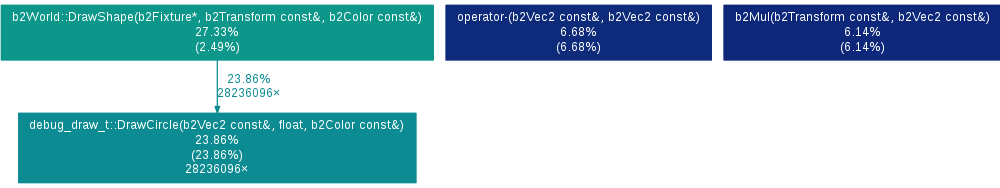
\includegraphics[width=1.05\textwidth]{1.png}
\end{figure}
\begin{figure}[H]
\caption{Callgraph-2}
\centering
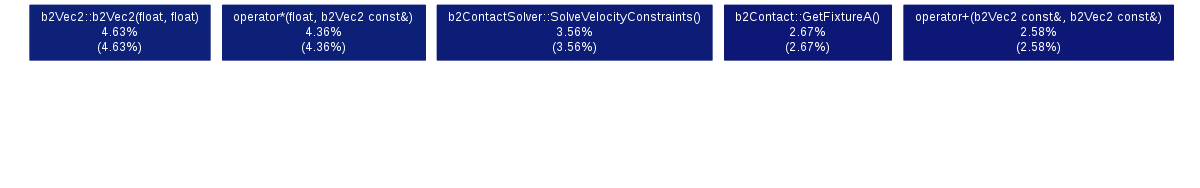
\includegraphics[width=1.05\textwidth]{2.png}
\end{figure}
\begin{figure}[H]
\caption{Callgraph-3}
\centering
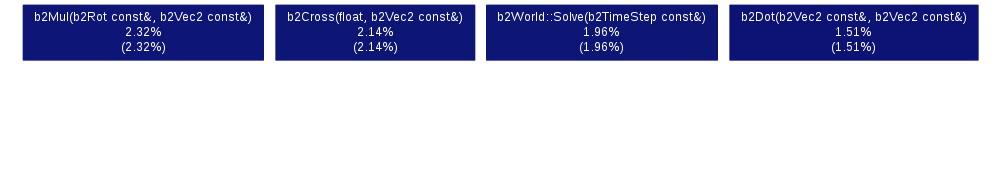
\includegraphics[width=1.05\textwidth]{3.png}
\end{figure}
\begin{figure}[H]
\caption{Callgraph-4}
\centering
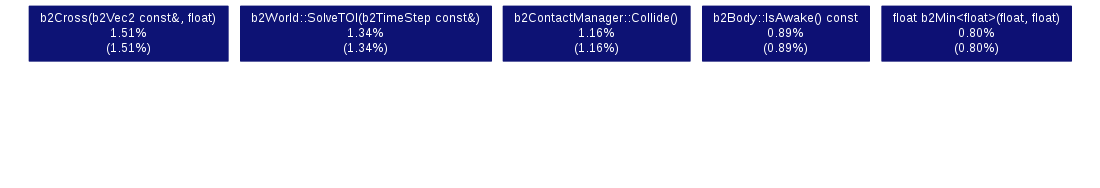
\includegraphics[width=1.05\textwidth]{4.png}
\end{figure}
\begin{figure}[H]
\caption{Callgraph-5}
\centering
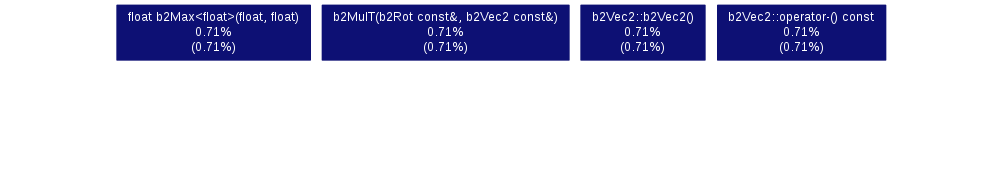
\includegraphics[width=1.05\textwidth]{5.png}
\end{figure}
\begin{figure}[H]
\caption{Callgraph-6}
\centering
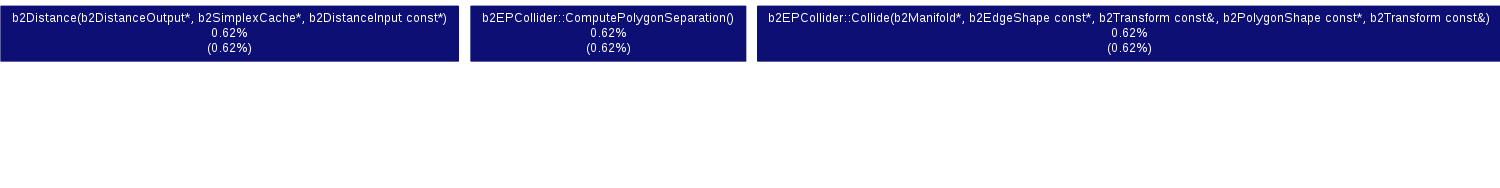
\includegraphics[width=1.05\textwidth]{6.png}
\end{figure}
\begin{figure}[H]
\caption{Callgraph-7}
\centering
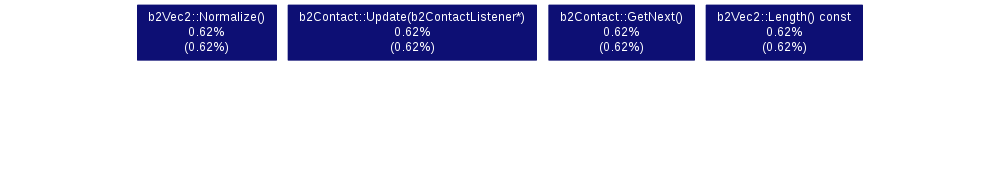
\includegraphics[width=1.05\textwidth]{7.png}
\end{figure}
\begin{figure}[H]
\caption{Callgraph-8}
\centering
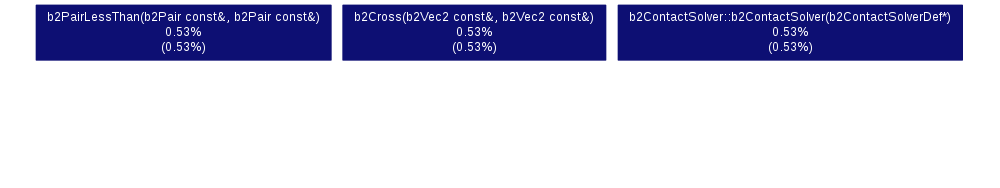
\includegraphics[width=1.05\textwidth]{8.png}
\end{figure}
\begin{figure}[H]
\caption{Callgraph-9}
\centering
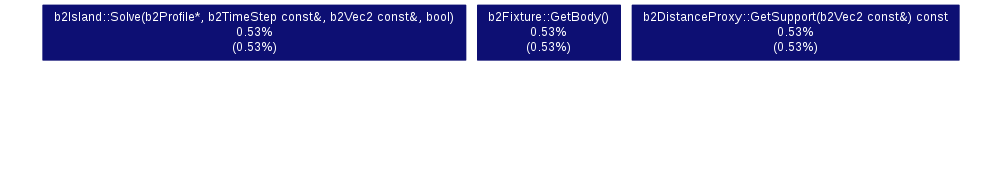
\includegraphics[width=1.05\textwidth]{9.png}
\end{figure}


\pagebreak 

\begin{thebibliography}{9}
\bibitem{ref1} 
IVARS PETERSON.
Riding on Square Wheels
\url{https://www.sciencenews.org/article/riding-square-wheels}
\bibitem{ref2}
FREYMAN ART.
Square Wheeled Bicycle on a Catenary Curve
\url{https://www.youtube.com/watch?v=0BtZcmEkFsI}
\bibitem{ref3}
ALLAN BISHOP.
Box2D Tutorials
\url{http://blog.allanbishop.com/tutorials/}
\bibitem{ref4}
Box2D Manual. 
\url{http://box2d.org/manual.pdf}
\bibitem{ref5}
Sourabh Ghurye.
cs251 Base code
\url{http://www.cse.iitb.ac.in/~sourabhghurye/box2d/html/}
\bibitem{ref6}
Box2d forum (Many links)
\url{http://box2d.org/forum}
\url{http://box2d.org/forum/viewtopic.php?f=19&t=9489}
\url{http://www.box2d.org/forum/viewtopic.php?f=3&t=7886}
\bibitem{ref7}
Stack overflow (Many Links) 
\url{http://stackoverflow.com/questions/14746312/spring-effect-in-box2djs}
\url{http://stackoverflow.com/questions/18118827/error-when-destroying-a-joint}
\bibitem{ref8}
DistanceJointDef
\url{https://libgdx.badlogicgames.com/nightlies/docs/api/com/badlogic/gdx/physics/box2d/joints/DistanceJointDef.html}
\bibitem{ref9}
Aamod
CS 296 Project
\url{http://www.cse.iitb.ac.in/~aamod/cs296/project/html/classcs296_1_1dominos__t.html}
\bibitem{ref10}
Iforce2D Box2D tutorials
\url{http://www.iforce2d.net/b2dtut/}
\bibitem{ref11}
Aman Goel
Box2D Project
\url{https://github.com/amangoeliitb/Box2D-project}
\bibitem{ref12}
Department of Mathematics, Computer Science, and Statistics, Bloomsburg University, Bloomsburg, Pennsylvania 17815.
50 Famous curves.
\url{https://elepa.files.wordpress.com/2013/11/fifty-famous-curves.pdf}
\bibitem{ref13}
ERIN CATTO
Box2D User Manual
\url{http://www.box2d.org/manual.html}
\bibitem{ref14}
SHARE LATEX
\url{www.sharelatex.com}
\bibitem{ref15}
 Iron Summit Media Strategies, LLC (2013-15)	
\url{https://github.com/IronSummitMedia/startbootstrap-freelancer/}
\end{thebibliography}

\end{document} 
